\section{Resumen de la solución propuesta} \label{sec:sol}
% indicarase a solución aportada para o problema
% presentado. Deberase incluír aquí a metodoloxía empregada.

    Tras una fase de investigación para determinar las bases del proyecto, limitaciones e información que es necesario recopilar en los servidores, se ha realizado una comparativa entre los principales lenguajes de programación creando una aplicación con funcionalidades mínimas (acceder a librerías del sistema). Estas actividades han permitido tomar las siguientes decisiones.
    
    Se creará un \textit{agente modular} utilizando el lenguaje de programación \textit{CSharp}, más concretamente \textit{.NET Framework} debido a la alta compatibilidad que brinda con las librerías de \textit{Windows}. Esto permitirá utilizar los mecanismos que proporciona el sistema operativo para obtener información propia.
    
    Los \textit{plugins} serán creados como librerías externas que podrán ser cargadas por el \textit{agente} en caso de estar en una carpeta específica durante su ejecución. La comunicación entre los \textit{plugins de entrada} y \textit{plugins de salida} se realizará mediante \textit{cadenas de texto} en formato \textit{JSON}, y ambos deberán recibir los parámetros necesarios en este mismo formato.
    
    Se utilizarán sistemas de control de versiones y se creará un repositorio para cada uno de los componentes, configurando mecanismos de \textit{integración continua} que permitan automatizar los procesos de compilación y publicación de nuevas versiones. Las publicaciones creadas proveerán con la información necesaria al sistema de actualización automática.
    
    El mecanismo de actualización automática se encargará de mantener actualizado al agente, cada uno de los \textit{plugins} y a sí mismo. Para esto, comprobará periódicamente la última versión estable disponible, si esta es superior a la que está instalada actualmente, la reemplazará. Dado que mientras los componentes de la aplicación están siendo utilizados no pueden ser modificados, el sistema de actualización será creado como una aplicación independiente encargada de terminar el proceso del agente, llevar a cabo la actualización, e iniciarlo una vez finalizado este.
    
    Los ajustes de la aplicación se establecerán en formato \textit{JSON}, separando las configuraciones en tres bloques: el actualizador, los eventos del sistema y los \textit{plugins}. En los dos últimos, la configuración de entrada recogerá los detalles de la configuración de salida, que incluirá, además de sus propias opciones, la frecuencia con la que se obtendrán los datos para transmitirlos por esa vía.
    
    En la figura \ref{fig:proposed-solution-diagram} se puede apreciar un diagrama resumen de la solución propuesta para la realización de este proyecto.
    
    \begin{figure}[h!]
    \centering
        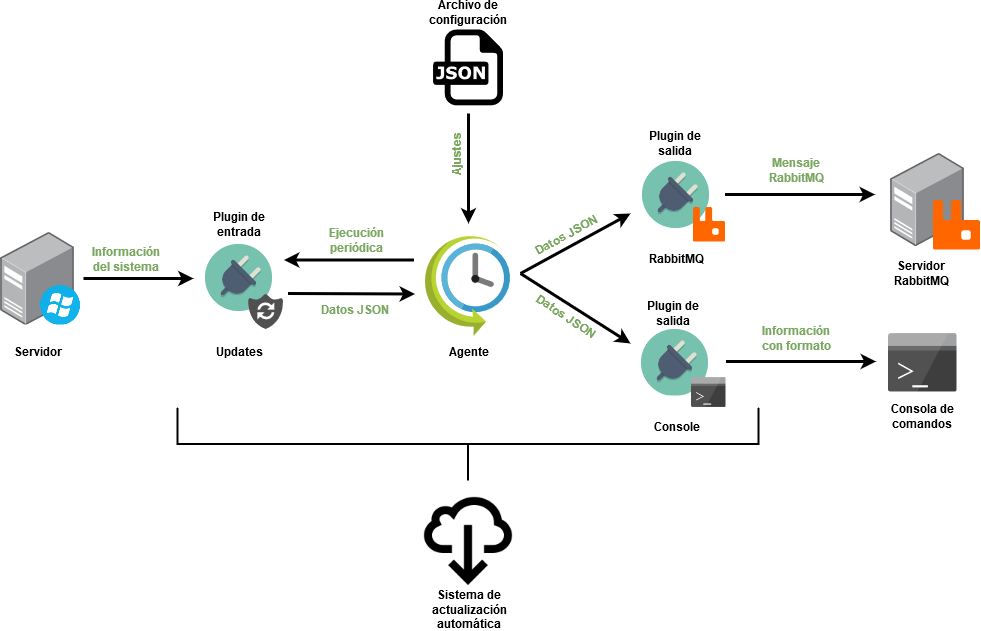
\includegraphics[scale=0.5]{diagrama-solucion-propuesta.png}
        \caption{Resumen de la solución propuesta}
        \label{fig:proposed-solution-diagram}
    \end{figure}
    
    Este proyecto parte de objetivos bien definidos y cierto nivel de detalle, sin embargo, una gran parte del sistema a desarrollar depende en su totalidad de librerías tanto de \textit{Windows} como de terceros. Esto es una limitación, y hace que la planificación inicial pueda variar debido a incompatibilidades entre ellas. Debido a esto se ha concluido que lo más adecuado sería el uso de un método ágil de desarrollo de software, en concreto \textit{SCRUM}, que está más enfocado a la administración del desarrollo iterativo. \textit{SCRUM} consta de tres fases:
        
    \begin{itemize}
        \item Planificación de un \textit{boceto}, donde se establecen los objetivos generales del proyecto y el diseño de la arquitectura del software.
        
        \item Una serie de ciclos \textit{sprint}, donde cada ciclo desarrolla un incremento del sistema.
        
        \item \textit{Cierre} del proyecto, fase en la cual se completa la documentación requerida como ayudas y manuales de usuario.
    \end{itemize}

    \textit{SCRUM} permite que el producto se desglose en piezas comprensibles de forma individual y que son desarrolladas de forma iterativa, recibiendo retroalimentación del usuario con cada entrega y realizando cambios en consecuencia. Para llevar a cabo el desarrollo utilizando este método, es necesario ocupar los roles imprescindibles para su funcionamiento.

    \begin{itemize}
        \item \textbf{Equipo de desarrollo:} Equipo responsable de llevar a cabo el desarrollo del sistema. Este rol estará compuesto únicamente por el alumno.
        
        \item \textbf{Cliente:} Encargado de definir los requisitos, utilizar las versiones resultantes de cada \textit{sprint} y aportar retroalimentación para la mejora del sistema. Este rol será llevado a cabo por el supervisor del proyecto.
        
        \item \textbf{Maestro de SCRUM:} Encargado de rastrear el trabajo que queda por hacer, tomar decisiones, medir el avance en función de la planificación inicial y mantener la comunicación con el cliente. Este rol será adoptado por el supervisor del proyecto.
    \end{itemize}
    
    
